\chapter{Технологический раздел}%
\label{cha:tekhnologicheskii_razdel}

В данном разделе производится выбор средств для разработки и рассматривается реализация программного обеспечения.

\section{Выбор языка программирования и среды разработки}%
\label{sec:vybor_iazyka_programmirovaniia_i_sredy_razrabotki}

В качестве языка программирования был выбран язык C, так как при помощи этого языка написано большинство загружаемых модулей ОС Linux.

В качестве текстового редактора был выбран текстовый редактор Vim.

Для автоматизации сборки была выбрана утилита make, а для компиляции~--- gcc.

Для перехвата функций ядра была выбрана библиотека khook.

\section{Некоторые моменты реализации}%
\label{sec:nekotorye_momenty_realizatsii}

Взаимодействие с пространством пользователя происходит при помощи механизма сигналов.

В листинге~\ref{lst:defsh} представлены объявления используемых в программе констант и типов. Здесь резервируются три определённых для пользователя сигнала, определяется структура linux\_dirent (оригинальное определение структуры было перемещено из соответствующего заголовочного файла в файл исходного текста ядра, поэтому доступ к нему был утерян).

Процесс в ОС Linux описывается структурой struct task\_struct, среди полей которой есть поле flags длиной 32 бит. Очевидно из названия, это поле предназначено для установки и сбрасывания флагов процесса. В листинге~\ref{lst:task_flags} представлены флаги task\_struct ядра версии 5.8.
\begin{lstlisting}[language=c,caption={Флаги task\_struct},label=lst:task_flags]
define PF_IDLE			    0x00000002	
#define PF_EXITING		    0x00000004	
#define PF_VCPU			    0x00000010	
#define PF_WQ_WORKER		0x00000020	
#define PF_FORKNOEXEC		0x00000040	
#define PF_MCE_PROCESS		0x00000080  
#define PF_SUPERPRIV		0x00000100	
#define PF_DUMPCORE		    0x00000200	
#define PF_SIGNALED		    0x00000400	
#define PF_MEMALLOC		    0x00000800	
#define PF_NPROC_EXCEEDED	0x00001000	
#define PF_USED_MATH		0x00002000	
#define PF_USED_ASYNC		0x00004000	
#define PF_NOFREEZE		    0x00008000	
#define PF_FROZEN		    0x00010000	
#define PF_KSWAPD		    0x00020000	
#define PF_MEMALLOC_NOFS	0x00040000	
#define PF_MEMALLOC_NOIO	0x00080000	
#define PF_LOCAL_THROTTLE	0x00100000	
#define PF_KTHREAD		    0x00200000	
#define PF_RANDOMIZE		0x00400000	
#define PF_SWAPWRITE		0x00800000	
#define PF_UMH			    0x02000000	
#define PF_NO_SETAFFINITY	0x04000000	
#define PF_MCE_EARLY		0x08000000  
#define PF_MEMALLOC_NOCMA	0x10000000	
#define PF_IO_WORKER		0x20000000	
#define PF_FREEZER_SKIP		0x40000000	
#define PF_SUSPEND_TASK		0x80000000  
\end{lstlisting}

Исходя из этого листинга можно сделать вывод, что не все разряды flags соответствуют тем или иным флагам. Поэтому, для того, чтобы установить, скрыт процесс или нет, зарезервируем один из свободных разрядов.

В листингах~\ref{lst:proc_h} и~\ref{lst:proc_c} описываются функции скрытия и отображения процессов. Эти функции проверяют и устанавливают/сбрасывают разряд переменной flags, определённый для индикации невидимости процесса.

Сетевые сокеты скрываются по номеру порта. Скрываемые порты хранятся в объявленном в листинге~\ref{lst:net_h} списке беркли. Определённые в листинге~\ref{lst:net_c} функции управляют содержимым этого списка.

Функции для перехвата tcp4\_seq\_show, tcp6\_seq\_show, udp4\_seq\_show, udp6\_seq\_show, getdents, getdents64 и kill определены в листинге~\ref{lst:rootkit_c}. Там же происходит скрытие и отображение модуля. Перехват функции kill требуется для обработки новых заданных сигналов.

\section{Апробация}%
\label{sec:aprobatsiia}

Рассмотрим примеры работы.

На рисунке~\ref{img:module_hide} демонстрируется сборка модуля, его загрузка, проверка скрытия и выгрузка.
\begin{figure}[H]
    \centering
    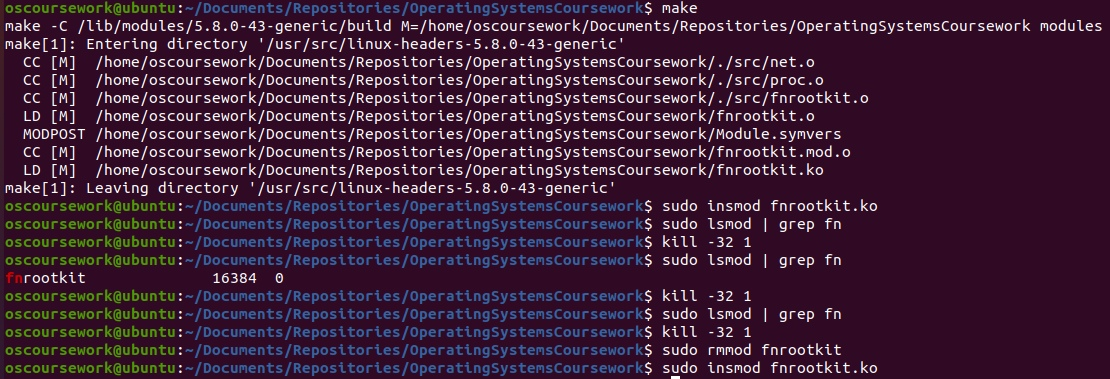
\includegraphics[scale=0.4]{images/scr_01.jpg}
    \caption{Загрузка, скрытие и выгрузка модуля}\label{img:module_hide}
\end{figure}

На рисунке~\ref{img:proc_hide} демонстрируется скрытие процесса.
\begin{figure}[H]
    \centering
    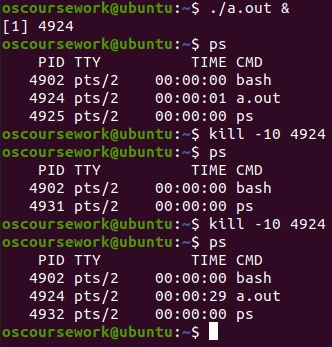
\includegraphics[scale=0.65]{images/scr_02.jpg}
    \caption{Скрытие процесса}\label{img:proc_hide}
\end{figure}

На рисунке~\ref{img:net_hide} демонстрируется скрытие сетевых сокетов.
\begin{figure}[H]
    \centering
    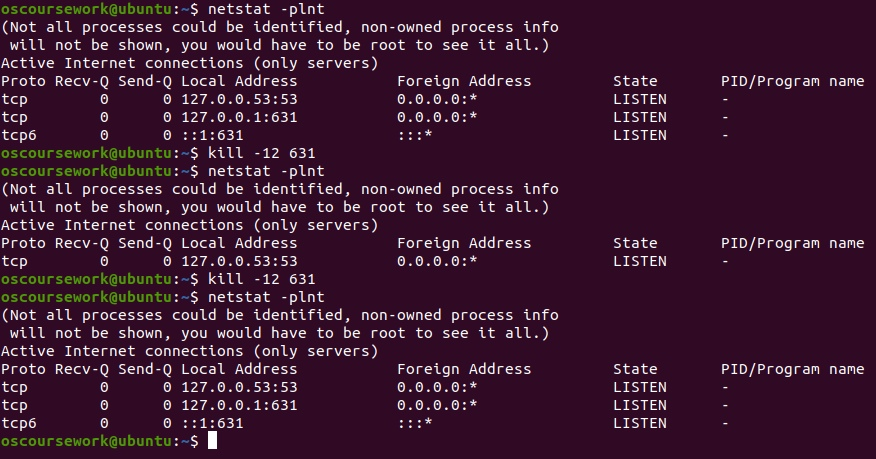
\includegraphics[scale=0.45]{images/scr_03.jpg}
    \caption{Скрытие сетевых сокетов}\label{img:net_hide}
\end{figure}

В ходе тестирования данного ПО не было выявлено ошибок.

\section{Выводы}%
\label{sec:vyvody}

В данном разделе был выбран язык программирования C, а также рассмотрена реализация программного обеспечения. Помимо этого, программное обеспечение было протестировано на наличие ошибок.
